%!TEX root = informe.tex
\chapter{El Análisis de Ciclo de Vida}
\section{Introducción}
La importancia de la protección medioambiental ha ido en creciente aumento en los últimos años \cite{iso14040}. El interés en los procesos de fabricación de los productos tanto manufacturados como consumidos y sus posibles impactos asociados han generado un nuevo campo de desarrollo de técnicas de análisis, entre las que se encuentra el Análisis de Ciclo de Vida (ACV).

Lo que distingue al ACV del resto de técnicas es que realiza un estudio a lo largo de todas las etapas de la vida de un producto, desde la obtención de la materia prima, pasando por la producción, uso, tratamiento final, reciclado, hasta su disposición final, de la ``cuna a la tumba'', abarcando tanto los aspectos ambientales como los impactos potenciales.

El Análisis de Ciclo de Vida sigue los siguientes protocolos estándar:
\begin{itemize}
\item UNE-EN-ISO 14040:2006, Gestión Ambiental. Análisis de ciclo de vida. Principios y marco de referencia.
\item UNE-EN-ISO 14440:2006, Gestión ambiental. Análisis de ciclo de vida. Requisitos y Directrices.
\item UNE-EN-ISO 150041EX:1998, Análisis de ciclo de vida simplificado.
\end{itemize}

El ACV utilizado como herramienta de gestión ambiental ayuda a identificar los recursos utilizados y los residuos emitidos a los vectores ambientales —emisiones atmosféricas, aguas residuales y suelo— a lo largo de todo el ciclo de vida, ya sea de un producto o un servicio \cite{iso14440}.

\section{Relación entre la construcción y el medioambiente}
El sector de la construcción es uno de los más productivos e importantes tanto social como económicamente. Las infraestructuras construidas aportan calidad de vida al ser humano. Como toda actividad humana, el desarrollo de esta actividad provoca impactos significativos en el medio tanto a la hora de producir, usar y eliminar sus productos.

La concienciación de protección del medio ha obligado al sector a mejorar sus actuaciones en esta materia sin disminuir su capacidad productiva para seguir siendo competitivos. Debe crearse un nuevo paradigma de trabajo en el que el usuario esté satisfecho, el consumo de materia y energía sea mínimo, así como el impacto medioambiental, pero a su vez mejorando la calidad y disminuyendo el tiempo y el coste \cite{carvalho}.

AUGENBROE, 1998.
ITeC, 2000.
SYMONDS, 1999.

El impacto medioambiental de un producto cambia según la etapa del ciclo de vida, produciendo diferentes efectos contaminantes sobre el entorno y sobre las personas. Sirva de ejemplos los siguientes datos \cite{carvalho}:
\begin{itemize}
\item el sector de la construcción moviliza un 10\% de la economía mundial y consume un 40\% de la energía mundial producida cada año.
\item según estudios realizados en varios países europeos entre los que se encuentra España, el consumo energético asociado al sector se distribuye en:
  \begin{itemize}
  \item 19\% para la construcción y mantenimiento de edificios.
  \item 48\% para el consumo directo debido a su uso (electricidad, gas, etc.).
  \item 33\% para el transporte.
  \end{itemize}
\item los residuos de la construcción y demolición (RCD) generados en la Unión Europea superan los 180 millones de toneladas cada año, es decir, 480 kg. por persona y año. De esos residuos, sólo el 28\% son reutilizados.
\end{itemize}

\section{Descripción del ciclo de vida de un producto de la construcción}
Una buena práctica para poder comprende mejor el ciclo de vida de un producto es la estructuración del sistema en procesos, de forma que queden representados todos los subsistemas constituyentes y se pueda identificar claramente un inicio y un final de cada uno.

Un diagrama que represente los flujos de entrada (materiales, energía, productos inacabados) y salida (productos finales, productos inacabados, co-productos, residuos) aporta una visión más clara de las fases del ciclo completo. Con los elementos bien identificados es más fácil atribuirle causas y consecuencias tanto a su subsistema como al sistema completo (ver figura \ref{fig:flujo_generico_acv}).

\begin{figure}[!htb]
\centering
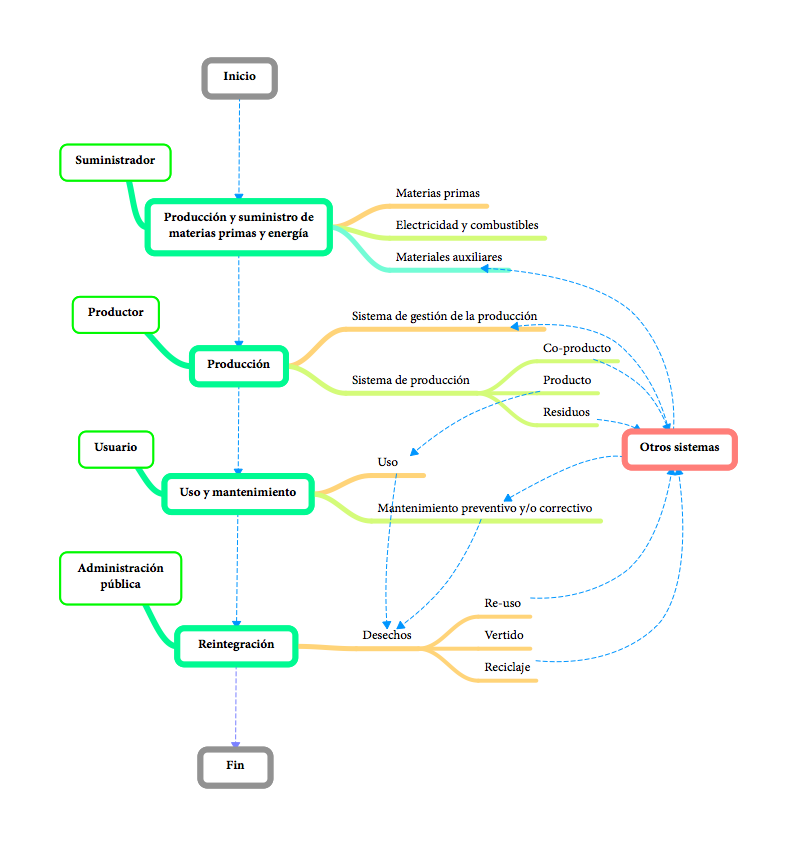
\includegraphics[width=15cm]{flujo_generico_acv.png}
\caption{Flujo genérico del ciclo de vida de un producto}
\label{fig:flujo_generico_acv}
\end{figure}

El adoquín se ajusta perfectamente a este esquema. BLA BLA BLA. BLA.

\section{Impactos potenciales del adoquín al medio ambiente}
A la hora de analizar los aspecto medioambientales de un sistema es necesario establecer diferentes niveles de análisis para poder establecer una estrategia de estudio, ya que a lo largo de la vida de un producto se pueden encontrar diferentes contextos.

\begin{figure}[!htb]
\centering
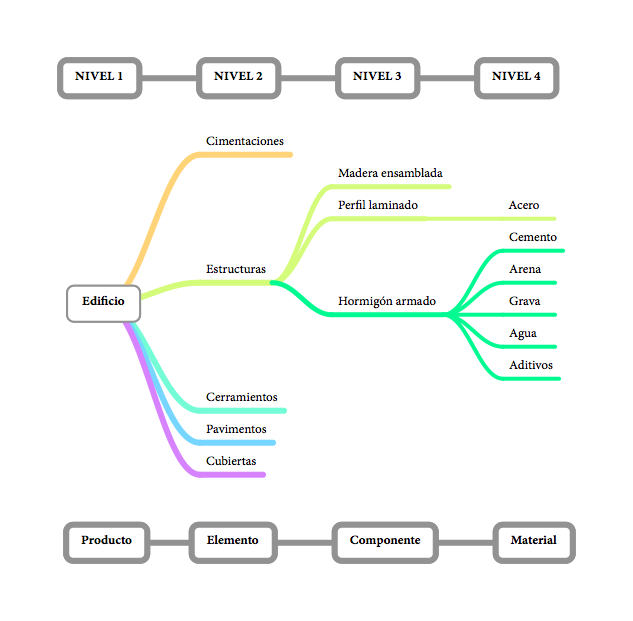
\includegraphics[width=15cm]{niveles_estudio_ciclo_vida.png}
\caption{Niveles de estudio del ciclo de vida.}
\label{fig:niveles_estudio_ciclo_vida}
\end{figure}

Al ser el adoquín un elemento de pavimentación se encontraría en el denominado nivel 2 (ver figura \ref{fig:niveles_estudio_ciclo_vida} ). Los impactos medioambientales del nivel 2 se clasifican según el momento de su vida en:

\begin{itemize}
  \item Producción
    \begin{itemize}
     \item Consumo de energía y recursos naturales en los procesos de producción y transporte.
     \item Producción de ruidos y vibraciones.
     \item Producción de residuos por excedentes de procesos y embalajes.
     \item Emisiones de partículas al aire (p. ej.: polvo).
    \end{itemize}
  \item Uso y mantenimiento
    \begin{itemize}
      \item Consumo de energía y recursos en los procesos de mantenimiento.
      \item Producción de residuos o sustancias tóxicas en función de los procesos de mantenimiento, su naturaleza y vida útil.
    \end{itemize}
  \item Reintegración
    \begin{itemize}
      \item Impactos potenciales traspuestos al producto final que lo utiliza.
    \end{itemize}
\end{itemize}

\section{Análisis de Ciclo de Vida. Proceso completo}

\section{SimaPro}
SimaPro es una herramienta profesional desarrollada por la empresa holandesa PRé Consultants para el Análisis de Ciclo de Vida más utilizada actualmente por la mayor parte de los consultores y la industria, apoyada en la investigación de materiales y elementos por parte institutos y universidades \cite{mgoedkoop}. Permite modelar ciclos de vida complejos y analizarlos de forma sistemática y transparente, ya que puede rastrearse el origen de todos los resultados de forma sencilla.

\begin{figure}[!htb]
\centering
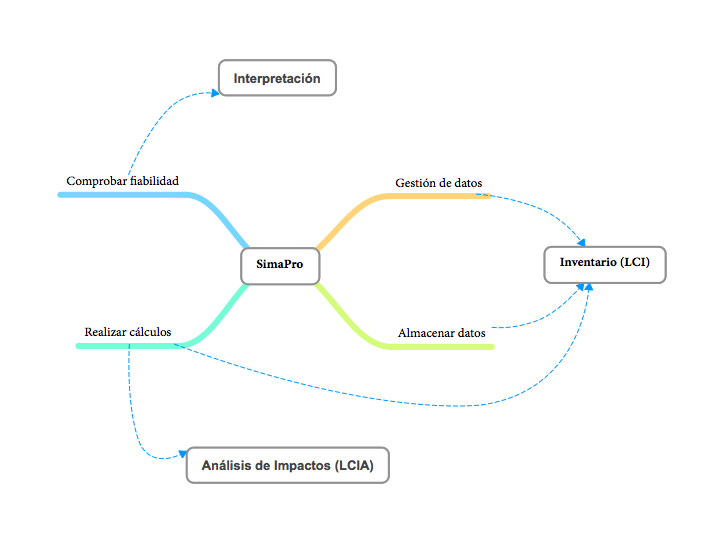
\includegraphics[width=15cm]{simapro.png}
\caption{Estructura de SimaPro.}
\label{fig:simapro}
\end{figure}

Entre sus principales cualidades destacan:

\begin{itemize}
  \item Diseño de productos.
  \item Desarrollo de indicadores clave.
  \item Cálculo de la huella de carbono de muchos tipos de productos y sistemas.
  \item Determinar el impacto medioambiental de productos o servicios con precisión estadística mediante el método de análisis Monte Carlo.
  \item Incluye Declaraciones Medioambientales de Productos e Informes Medioambientales GRI (Global Reporting Initiative).
  \item Utilización de bases de datos con inventarios.
  \item Asignación de múltiples procesos de salida.
  \item Análisis de Punto Débil, que permite identifica los puntos sensibles en el ciclo de vida utilizando un árbol de procesos.
  \item Análisis de tratamientos de residuos y escenarios de reciclado.
\end{itemize}

Esta herramienta cuenta con una interfaz de usuario intuitiva con un explorador de guía a través del Análisis de Ciclo de Vida del producto o servicio siguiendo los principios de las normas ISO 14040 y 14044. Además incorpora un modelado utilizando un asistente paso a paso.

La mayor ventaja de esta herramienta es la utilización de bases de datos con los inventarios de miles de procesos y métodos más importante de análisis de impacto.

\subsection{Bases de datos en SimaPro}
SimaPro incluye varias bases de datos de inventarios con miles de procesos, además de los métodos de análisis de impacto más importantes. De esta forma, no es necesario recolectar datos de procesos individuales y poder centrarse en los asuntos más importantes del estudio.

\begin{figure}[!htb]
\centering
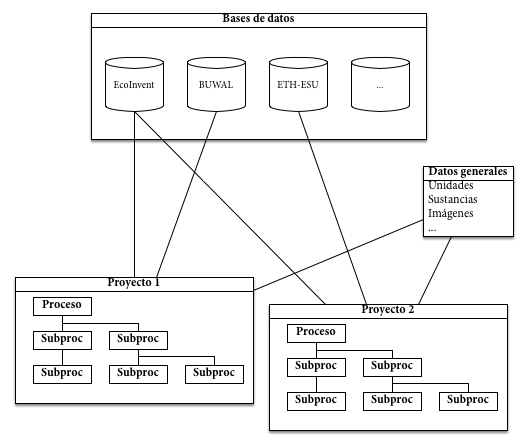
\includegraphics[width=15cm]{bbddsimapro.png}
\caption{Estructura de una base de datos de SimaPro.}
\label{fig:bbddsimapro}
\end{figure}

La calidad de los datos que aparecen en el Inventario de Ciclo de Vida (ICV) implica que el estudio sea relevante o no. \textit{ecoinvent} implementa en una única base de datos miles de conjuntos de datos de ICVs —agricultura, energía, transporte, combustibles, biomateriales, químicos, materiales de construcción, materiales de empaquetamiento, metales elementales y preciosos, procesado de metales, informática y electrónica, tratamiento de residuos— basados en información industrial recopilada por grupos de investigación y consultores reconocidos internacionalmente \cite{website:ecoinvent}.

\begin{figure}[!htb]
\centering
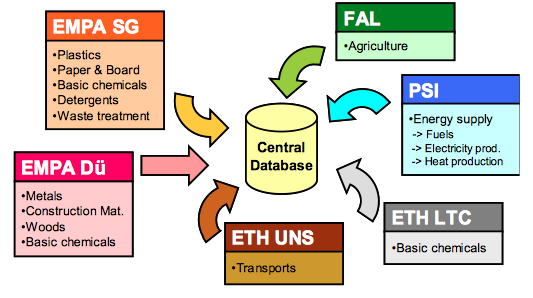
\includegraphics[width=15cm]{bbddecoinvent.png}
\caption[Estructura de la base de datos de \textit{ecoinvent}.]{Estructura de la base de datos de \textit{ecoinvent}. Fuente: \protect\cite{mgoedkoop2}.}
\label{fig:bbddecoinvent}
\end{figure}

De esta forma, la metodología de uso de SimaPro consiste en utilizar \textit{ecoinvent} como soporte para aquellos materiales y procesos de nuestro sistema que sean similares con los de la base de datos. En caso de que no se adapten a la entrada de la base de datos será necesario modelar una nueva entrada equivalente, pudiendo usar otras entradas de la base de \textit{ecoinvent}.

La librería \textit{ecoinvent}:
\begin{itemize}
  \item Incorpora más de 4000 procesos:
  \begin{itemize}
    \item Bienes de producción y calidades.
    \item Para algunos procesos añade diferencias regionales (Suiza y Unión Europea).
    \item Mix eléctrico y procesos agrícolas de Estados Unidos y Asia.
  \end{itemize}
  \item Incertidumbre en los datos.
  \item Ilustraciones de la mayoría de los procesos.
  \item Documentación extensa y consistente de los procesos.
  \item Actualizaciones frecuentes y periódicas.
  \item Incluye versiones de los procesos como Unidad (Proceso 1/U) —más detallado— o como Sistema (Proceso 1/S) —sin información de incertidumbre—.
\end{itemize}

\section{ReCiPe}\label{sec:recipe}

XXXX
